\subsection{Arduino}
	\par
		Arduino es una plataforma de electrónica de código abierto basada en hardware y software fácil de usar. Las placas Arduino pueden leer entradas (luz en un sensor, un dedo en un botón o un mensaje de Twitter) y convertirlo en una salida, activar un motor, encender un LED y publicar algo en línea. Puede decirle a su placa qué hacer enviando un conjunto de instrucciones al microcontrolador en la placa. Para hacerlo, utiliza el lenguaje de programación Arduino (basado en ``Wiring") y el software Arduino (IDE), basado en ``Processing"
	\par \noindent
		Con los años, Arduino ha sido el cerebro de miles de proyectos, desde objetos cotidianos hasta complejos instrumentos científicos. Una comunidad mundial de fabricantes (estudiantes, aficionados, artistas, programadores y profesionales) se ha reunido en torno a esta plataforma de código abierto, sus contribuciones se han añadido a una increíble cantidad de conocimiento accesible que puede ser de gran ayuda para principiantes y expertos por igual.
	\par \noindent
		Arduino nació en el Ivrea Interaction Design Institute como una herramienta fácil para el prototipado rápido, dirigido a estudiantes sin experiencia en electrónica y programación. Tan pronto como llegó a una comunidad más amplia, la placa Arduino comenzó a cambiar para adaptarse a las nuevas necesidades y desafíos, diferenciando su oferta de simples placas de 8 bits para productos para aplicaciones IoT, wearable, impresión 3D y entornos integrados. Todos los tableros Arduino son completamente de código abierto, lo que permite a los usuarios construirlos de forma independiente y eventualmente adaptarlos a sus necesidades particulares. El software también es de código abierto y está creciendo a través de las contribuciones de los usuarios en todo el mundo.
	\begin{figure}[h]
		\centering
		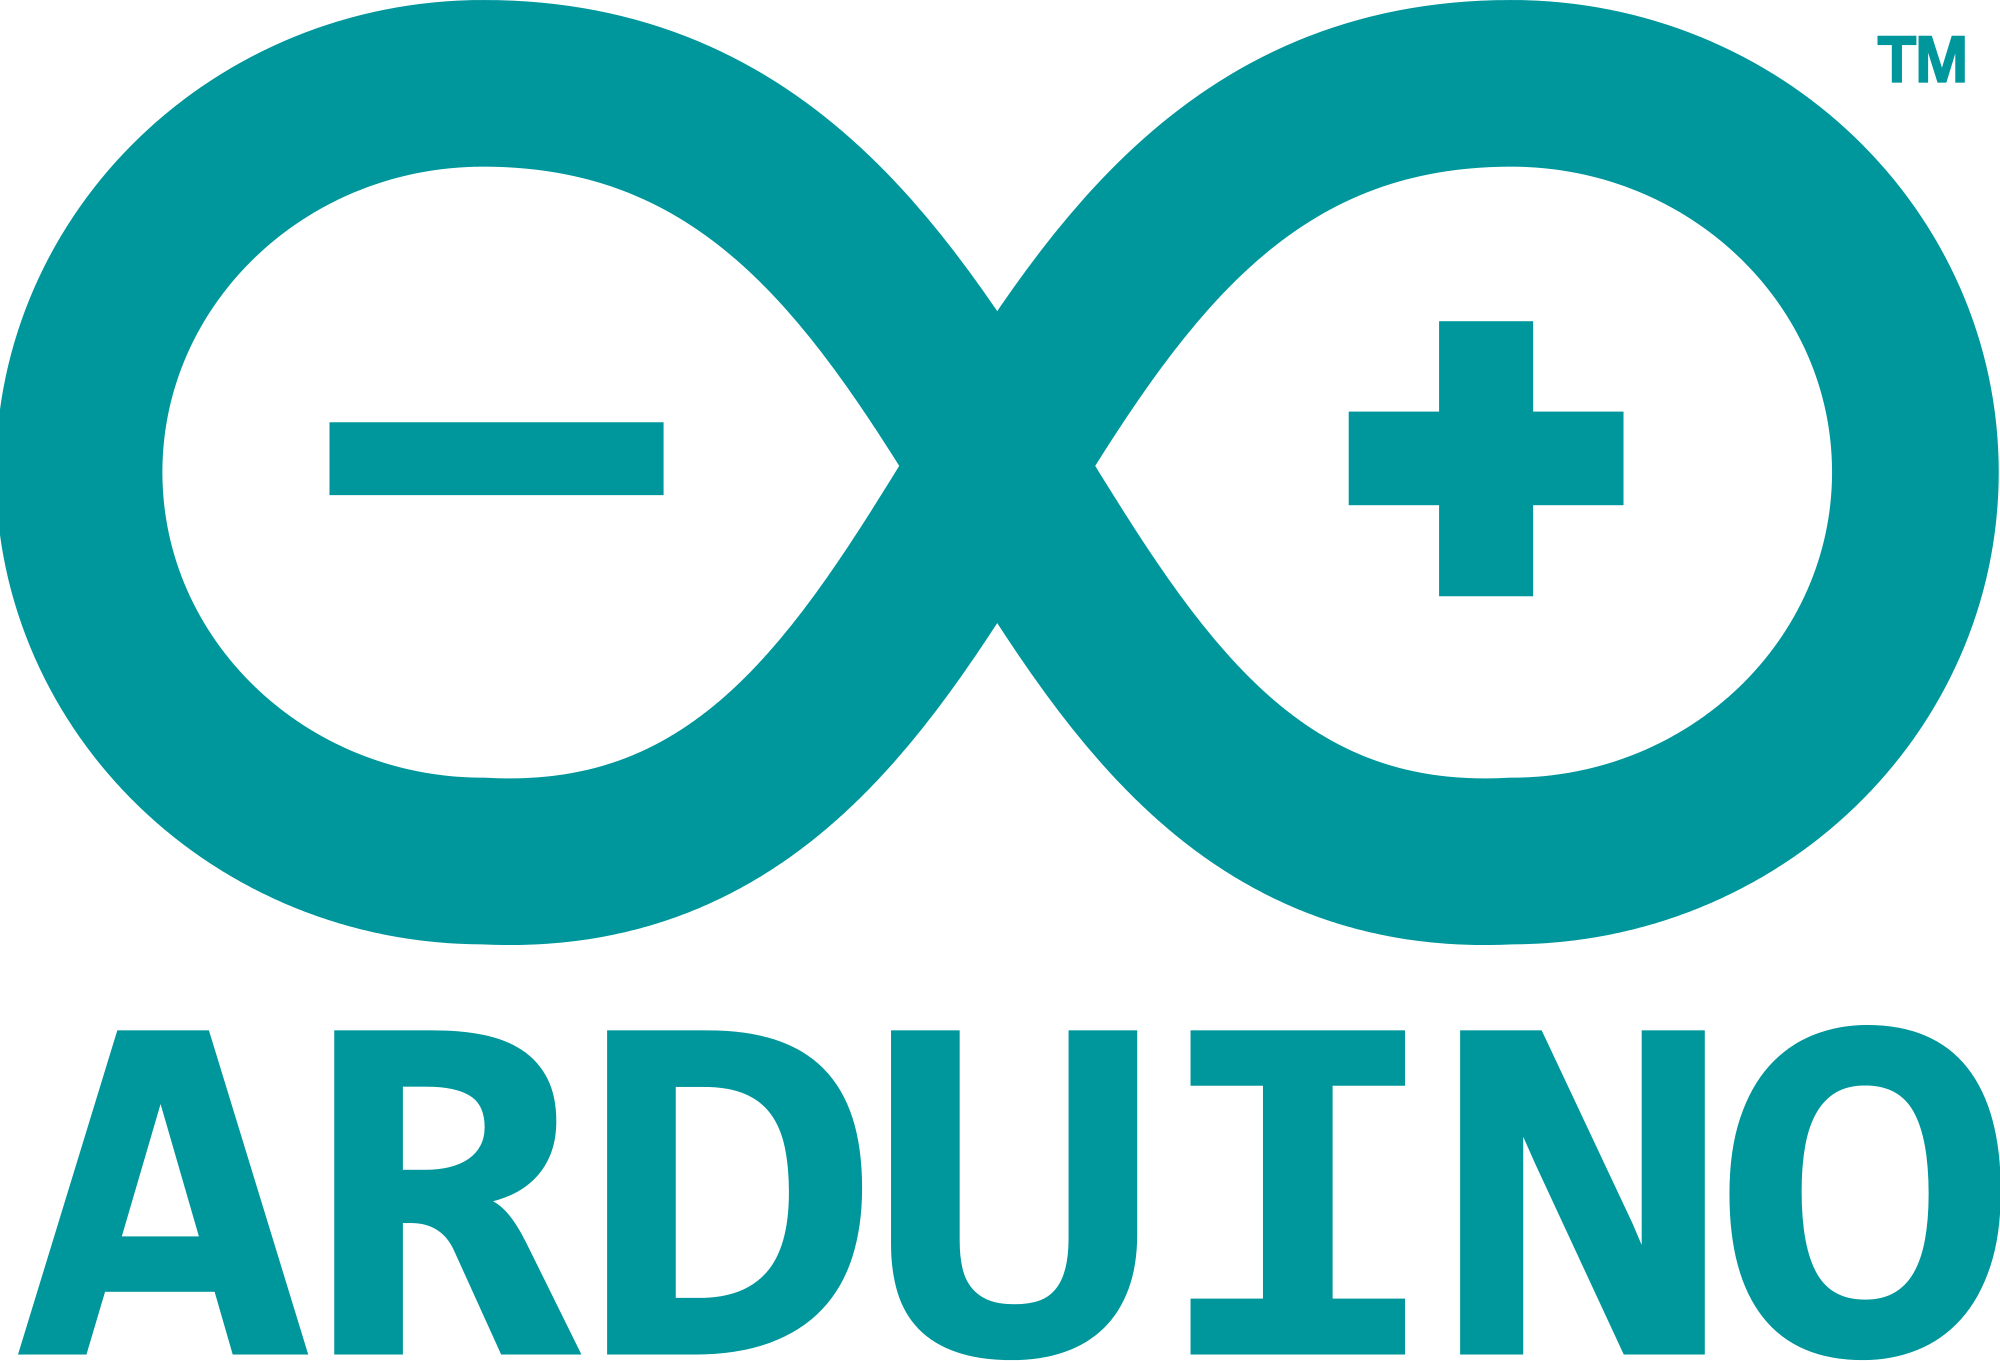
\includegraphics[width=0.4\textwidth]{figura5_arduinologo.png}
		\caption{Logo del proyecto de codigo abierto Arduino}
	\end{figure}

\newpage
\thispagestyle{plain}


	\subsubsection{Razones para utilizar Arduino}
		\begin{itemize}
			\item Económico: 
			Las placas Arduino son relativamente económicas en comparación con otras plataformas de microcontroladores. La versión menos costosa del módulo Arduino se puede ensamblar a mano, e incluso los módulos Arduino premontados cuestan menos de \$50.
			
			\item Multiplataforma: El software Arduino (IDE) se ejecuta en sistemas operativos Windows, Macintosh OSX y Linux. La mayoría de los sistemas de microcontroladores están limitados a Windows.
			
			\item Ambiente de Programación Sencilla: El software Arduino (IDE) es fácil de usar para principiantes, pero lo suficientemente flexible como para que los usuarios avanzados puedan aprovecharlo también. Para los maestros, está convenientemente basado en el entorno de programación de Procesamiento, por lo que los estudiantes que aprenden a programar en ese entorno estarán familiarizados con el funcionamiento del IDE de Arduino, adicional el lenguaje de programación es muy parecida a la C++.
			
			\item Software Extensible: El software Arduino se publica como herramientas de código abierto, disponibles para la extensión por programadores experimentados. El lenguaje puede expandirse a través de bibliotecas C ++, y las personas que quieran comprender los detalles técnicos pueden dar el salto de Arduino al lenguaje de programación AVR C en el que se basa. Del mismo modo, puede agregar código AVR-C directamente en sus programas Arduino si así lo desea.
			
			\item Hardware Extensible: 
			Los planes de las placas Arduino se publican bajo una licencia de Creative Commons, por lo que los diseñadores de circuitos experimentados pueden hacer su propia versión del módulo, ampliarlo y mejorarlo. Incluso los usuarios relativamente inexpertos pueden construir la versión del módulo para comprender cómo funciona y ahorrar dinero.
		\end{itemize}